\section{Interpretation}
\label{sec:Interpretation}

In this section we will explain how to interpret a trace view once it has been adjusted as 
described in the previous section.

\begin{itemize}
 \item The trace view has in its horizontal axis the execution time and in the vertical 
       axis one line for the master at the top, and below it, one line for each of the workers.
 \item In a line, the light blue color means idle state, in the sense that there is no event at that time.
 \item Whenever an event starts or ends a flag is shown.
 \item In the middle of an event, the line shows a different color. Colors are assigned depending on the event type.
 \item In the info panel the legend of assigned color to event type is provided.
\end{itemize}

\begin{figure}[ht!]
  \centering
    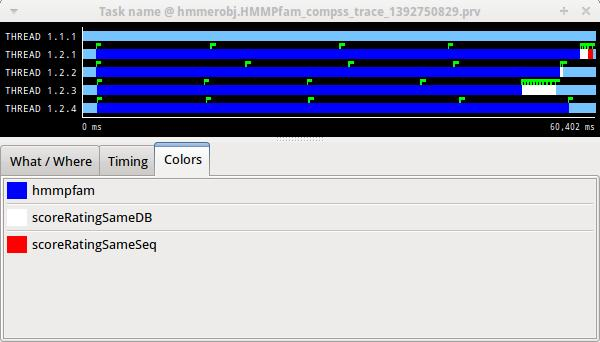
\includegraphics[width=\textwidth]{./Sections/4_Interpretation/Figures/7.jpeg}
    \caption{Trace interpretation}
\end{figure}